\section{Classification}

Instead of predicting $y \in \R$, we limit $y$ to be in a finite, discrete set $Y$ (e.g. $\{-1, +1\}$). When looking at binary classification we often use the labels $-1, +1$ and let the predicted value be equal to $\hat{y} = \sgn\hat{f}(x)$. Similar to regression we care about the generalization error:
$$R(\hat{f}) = \mathbb{P}_{x,y} [y \neq \sgn \hat{f}(x)] = \E_{x,y}[\ell_{0-1}(\hat{f}(x), y)]$$

Where we call $\ell_{0-1}(\hat{f}(x), y) = \mathbb{I}_{y \neq \sgn \hat{f}(x)}$ the \textbf{zero-one loss}. Since this loss is neither convex nor continuous, we can not efficiently minimize the training error with it. Therefore we introduce different type of loss functions:
\begin{itemize}
	\item \textbf{Exponential loss}: $\ell_\text{exp}(\hat{f}(x), y) = e^{y \hat{f}(x)}$
	\item \textbf{Logistic loss}: $\ell_\text{log}(\hat{f}(x), y) = \log(1 + e^{y \hat{f}(x)})$
	\item \textbf{Hinge loss}: $\ell_\text{hinge}(\hat{f}(x), y) = \max(0, 1-y \hat{f}(x))$
	\item \textbf{Linear loss}: $\ell_\text{lin}(\hat{f}(x), y) = y \hat{f}(x)$
\end{itemize}

We will mainly focus on the logistic loss (also called \textbf{logistic regression}), as in practice it is the most used. We can derive that the logistic loss is the negative conditional $\log$ likelihood $\mathbb{P}[y = +1 | x]$ or $\mathbb{P}[y = -1 | x]$ that is parameterized by $\hat{f}(x)$ via the \textbf{softmax transformation}. We define (similar for $y = -1$): $$\mathbb{P}[y = +1 | x] = \frac{1}{1 + e^{- \hat{f}(x)}}$$

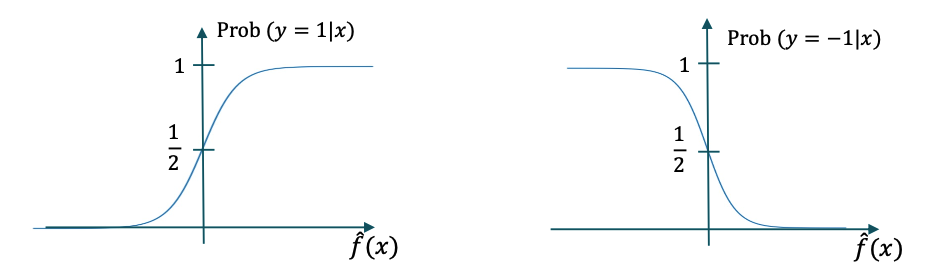
\includegraphics[width=\columnwidth]{conditional-probability.png}

Using this we can define the probability vector:
$$\hat{p}(x) = (\mathbb{P}[y = -1 | x], \; \mathbb{P}[y = +1 | x])$$

If we want to extend the log loss to multiple classes, we define a vector $\tilde{f}(x) = (\hat{f}_1(x), ..., \hat{f}_K(x))$ and transform it using softmax:
$$\hat{p}_k = \frac{e^{\hat{f}_k(x)}}{\sum_{i=1}^K e^{\hat{f}_j(x)}}$$

For the multiclass case we choose the classifier error to be the maximal entry of $\hat{p}$ if $y \neq \hat{y}$.

\subsection{Linear Classifiers}

Linear classifiers use functions form the class $F = \{ f \; | \; f(x) = w^\top x, \; w \in \R^d\}$. We already know that this class of functions makes training and prediction simple. The decision boundary of the function is given by $\{ x \; | \; f(x) = 0\}$.

\begin{center}
	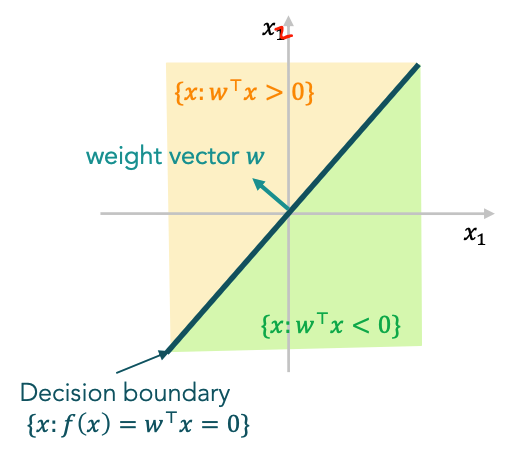
\includegraphics[width=0.64\columnwidth]{linear-classifiers.png}
\end{center}

To train our classifier we can use gradient descent. The gradient of the logistic loss is given by:
$$\nabla \ell(\hat{f}(x), y) = \frac{y_i x_i}{1 + e^{y_i \hat{f}(x)}}$$
 
 For linearly separable data, gradient descent on the logistic loss converges to the direction $w_\text{MM}$ that maximizes the minimum $\ell_2$-distance between the decision boundary and $y_i$. We call this the \textbf{maximum-margin} solution.
 
 In particular we can write:
 $$w_\text{MM} = \argmax{||w||_2 = 1} \min_i y_i w^\top x_i = \argmax{||w||_2 = 1} \; \text{margin} (w)$$
 
 Instead of just linear functions, we can again use feature mapping to receive nonlinear classifiers.
 
 \subsection{Support Vector Machines}
 
 For general $w$ that correctly separates the data, $\frac{\text{margin}(w)}{||w||_2}$ is the min. distance of any point to the decision boundary. If we use general $w$ the solution is not unique anymore. But we can rescale any unit norm $w$ by $\alpha = \frac{1}{\text{margin}(w)}$ such that $\alpha w = \tilde{w}$. So instead of searching within unit norm $w$ to find $w_\text{MM}$ with maximum margin, we can search within all $\tilde{w}$ with margin$(\tilde{w}) = 1$ to find the one that maximizes:
 $$\frac{\text{margin}(\tilde{w})}{||\tilde{w}||_2} = \frac{1}{||\tilde{w}||_2}$$ 
 
 This is how support vector machines work. More formal:
 $$\hat{w} = \min_w ||w||_2 \quad \text{s.t. } y_i w^\top x_i \geq 1 \text{ for all } i=1,...,n$$
 
 If the data is not linearly separable, we might want to use a \textbf{soft-margin SVM}. Since not all constraints can hold, we want to allow some "slack" in the constraints:
 
  $$\hat{w} = \min_{w, \xi} \frac{1}{2} ||w||_2^2 + \lambda \sum_{i=1}^n \max (0, 1 - y_i w^\top x_i)$$
  
  The later part penalizes any margin violations. To find the optimal $\lambda$ one might use cross-validation.
  